\documentclass[a4 paper]{article}
\usepackage[inner=2.0cm,outer=2.0cm,top=2.5cm,bottom=2.5cm]{geometry}
\usepackage{setspace}
\usepackage[ruled]{algorithm2e}
\usepackage[rgb]{xcolor}
\usepackage{verbatim}
\usepackage{subcaption}
\usepackage{amsgen,amsmath,amstext,amsbsy,amsopn,tikz,amssymb}
\usepackage{fancyhdr}
\usepackage[colorlinks=true, urlcolor=blue,  linkcolor=blue, citecolor=blue]{hyperref}
\usepackage[colorinlistoftodos]{todonotes}
\usepackage{rotating}
\usepackage{booktabs}
\usepackage{float}
\usepackage{listings}
\newcommand{\ra}[1]{\renewcommand{\arraystretch}{#1}}

\newtheorem{thm}{Theorem}[section]
\newtheorem{prop}[thm]{Proposition}
\newtheorem{lem}[thm]{Lemma}
\newtheorem{cor}[thm]{Corollary}
\newtheorem{defn}[thm]{Definition}
\newtheorem{rem}[thm]{Remark}
\numberwithin{equation}{section}

\newcommand{\homework}[6]{
	\pagestyle{myheadings}
	\thispagestyle{plain}
	\newpage
	\setcounter{page}{1}
	\noindent
	\begin{center}
		\framebox{
			\vbox{\vspace{2mm}
				\hbox to 6.28in { {\bf MATH 118:~Statistics and Probability \hfill {\small (#2)}} }
				\vspace{6mm}
				\hbox to 6.28in { {\Large \hfill #1  \hfill} }
				\vspace{6mm}
				\hbox to 6.28in { {\it Instructor: {\rm #3} \hfill Name: Aygün Bayır {\rm #5} \hfill Student Id: 161044119 {\rm #6}} \hfill}
				\hbox to 6.28in { {\it Assistant: #4  \hfill #6}}
				\vspace{2mm}}
		}
	\end{center}
	\markboth{#5 -- #1}{#5 -- #1}
	\vspace*{4mm}
}

\newcommand{\problem}[2]{~\\\fbox{\textbf{Problem #1}}\hfill (#2 points)\newline\newline}
\newcommand{\subproblem}[1]{~\newline\textbf{(#1)}}
\newcommand{\D}{\mathcal{D}}
\newcommand{\Hy}{\mathcal{H}}
\newcommand{\VS}{\textrm{VS}}
\newcommand{\solution}{~\newline\textbf{\textit{(Solution)}} }

\newcommand{\bbF}{\mathbb{F}}
\newcommand{\bbX}{\mathbb{X}}
\newcommand{\bI}{\mathbf{I}}
\newcommand{\bX}{\mathbf{X}}
\newcommand{\bY}{\mathbf{Y}}
\newcommand{\bepsilon}{\boldsymbol{\epsilon}}
\newcommand{\balpha}{\boldsymbol{\alpha}}
\newcommand{\bbeta}{\boldsymbol{\beta}}
\newcommand{\0}{\mathbf{0}}


\begin{document}
	\homework{Homework \#2}{Due: 07/06/21}{Dr. Zafeirakis Zafeirakopoulos}{Gizem S\"ung\"u}{}{}
	\textbf{Course Policy}: Read all the instructions below carefully before you start working on the assignment, and before you make a submission.
	\begin{itemize}
		\item It is not a group homework. Do not share your answers to anyone in any circumstance. Any cheating means at least -100 for both sides. 
		\item Do not take any information from Internet.
		\item No late homework will be accepted. 
		\item For any questions about the homework, send an email to gizemsungu@gtu.edu.tr.
		\item Submit your homework (both your latex and pdf files in a zip file) into the course page of Moodle.
		\item Save your latex, pdf and zip files as "Name\_Surname\_StudentId".\{tex, pdf, zip\}.
		\item The answer which has only calculations without any formula and any explanation will get zero. 
		\item The deadline of the homework is 07/06/20 23:55.
		\item I strongly suggest you to write your homework on \LaTeX. However, hand-written paper is still accepted \textbf{IFF} your hand writing is \textbf{clear and understandable to read}, and the paper is well-organized. Otherwise, I cannot grade your homework.
		\item You do not need to write your Student Id on the page above. I am checking your ID from the file name.
	\end{itemize}
	
	\problem{1:}{10+10+10+10+10+10+40 = 100}
	\textbf{WARNING:} Please show your OWN work. Any cheating can be easily detected and will not be graded.
	\newline
	\newline
	For the question, please follow the file called manufacturing\_defects.txt while reading the text below.\\
	\newline
	In each year from 2000 to 2019, the number of manufacturing defects in auto manufacturers were counted. The data was collected from 14 different auto manufactory companies. The numbers of defects for the companies are indicated in 14 columns following the year column. Assume that the number of manufacturing defects per auto company per year is a random variable having a Poisson($\lambda$) and that the number of defects in different companies or in different years are independent.\\
	(Note: You should implement a code for your calculations for each following subproblem. You are free to use any programming languages (Python, R, C, C++, Java) and their related library.)
	
	\subproblem{a} Give a table how many cases occur for all companies between 2000 and 2019 for each number of defects (\# of Defects).\\
	Hint: When you check the file you will see: \# of Defects = \{0, 1, 2, 3, 4\}.\\
	\begin{table}[H]
		\centering
		\begin{tabular}{c|c}
			\begin{tabular}[c]{@{}c@{}}\textbackslash{}\# of\\Defects\end{tabular} & \begin{tabular}[c]{@{}c@{}}\textbackslash{}\# of cases\\in all company \\between the years\end{tabular}  \\ 
			\hline
			0 & 144 \\
			1 & 91 \\
			2 & 32 \\
			3 & 11 \\
			4 & 2 \\                                                                                                       
		\end{tabular}
		
		\caption{Actual cases}
		\label{tab1}
	\end{table}
	
	\subproblem{b} Estimate $\lambda$ from the given data. \\
	$\lambda$ = 0.7 \\
	
	\subproblem{c} Update Table \ref{tab1} in Table \ref{tab2} with Poisson predicted cases with the estimated $\lambda$.\\
	\begin{table}[H]
		\centering
		\begin{tabular}{c|c|c}
			\begin{tabular}[c]{@{}c@{}}\textbackslash{}\# of\\Defects\end{tabular} & \begin{tabular}[c]{@{}c@{}}\textbackslash{}\# of cases\\in all companies\\between the years\end{tabular} & \begin{tabular}[c]{@{}c@{}}Predicted \textbackslash{}\# of cases\\in all companies\\between the years\end{tabular}  \\ 
			\hline
			0 & 144 & 139.04 \\
			1 & 91 & 97.33 \\
			2 & 32 & 34.07 \\
			3 & 11 & 7.95 \\
			4 & 2 & 1.39 \\            
		\end{tabular}
		\caption{Actual vs. Predicted Cases}
		\label{tab2}
	\end{table}
	\subproblem{d} Draw a barplot for the actual cases (Table \ref{tab2} in column 2) and the predicted cases (Table \ref{tab2} column 3) with respect to \# of defecrs. You should put the figure.\\
	
	
	
	\begin{figure}[H]
		\centering
		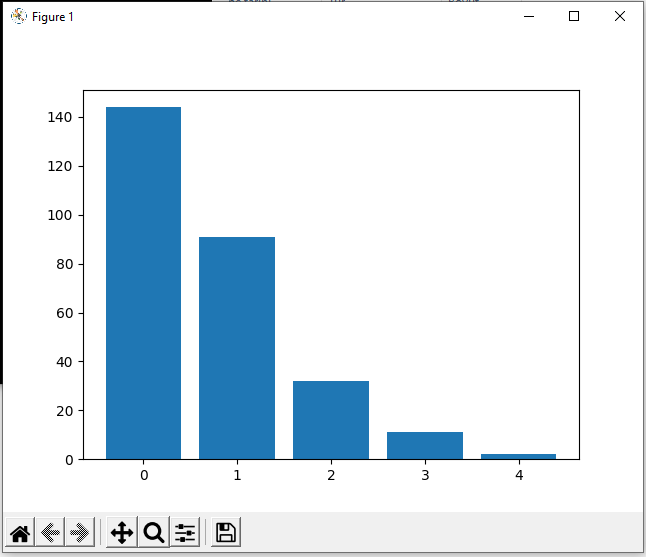
\includegraphics[width=0.7\linewidth]{1}
		\caption{Number of defects}
		\label{fig:1}
	\end{figure}

	\begin{figure}[H]
		\centering
		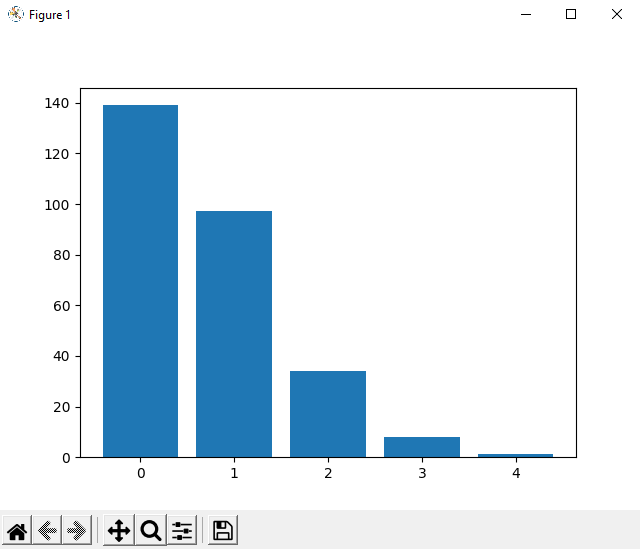
\includegraphics[width=0.7\linewidth]{2}
		\caption{Predicted number of defects}
		\label{fig:2}
	\end{figure}
	
	
	
	
	\subproblem{e} According to the barplot in (c), does the poisson distribution fit the data well? Compare the values of the actual cases and the values of the poisson predicted cases, and write your opinions about performance of the distribution.\\
	
	Predicted number of cases which we get by using poisson distribution are very close to our data. I can say it fit the data very well. For example, for zero, number of cases is 144 and predicted number is 139.04 which is very close to number of cases. I honestly say that poisson distribution give us numbers that are approximately 5 percent more or less to our data numbers which is very fine. \\
	
	\subproblem{f} According to your estimations above, write your opinions considering your barplot and Table \ref{tab2}. Do you think that road transportation is dangerous for us? Whether yes or no, explain your reason. \\
	
	I can say that no, road transportation is not dangerous for us. Since we know that every year, car companies produce millions of cars and we see in our data there are only tens or hundreds of manufacturing defects are happenning. It is very small numbers for these kind of big number of productions. So, margin of error is very low. Therefore I can say that road transportation is very safe. \\
	
	\subproblem{g} Paste your code that you implemented for the subproblems above. Do not forget to write comments on your code.\\
	Example:\\
	\begin{itemize}
		\item The common code block for all subproblems\\
		Paste here. Your code should read the file and compute other things which the following subproblems need.

		\lstset{language=Python}
		\lstset{frame=lines}
		\lstset{caption={Common part}}
		\lstset{label={lst:code_direct}}
		\lstset{basicstyle=\footnotesize}
		\begin{lstlisting}
		# import csv library for reading text file
		import csv
		with open('manufacturing_defects.txt', 'r') as file:
		reader = csv.reader(file, delimiter='\t') # all values are seperated with tab
		data = list(reader)
		
		# import matplotlib library for drawing barplot
		import matplotlib.pyplot as plt
		
		# Function to calculate factorial of number n
		def factorial(n):
		if n == 0:
		return 1
		else:
		return n * factorial(n-1)
		\end{lstlisting}

		\item The code block for (a)\\
		Paste here. Your code should compute the values in Table \ref{tab1} column 2.
		\lstset{language=Python}
		\lstset{frame=lines}
		\lstset{caption={Part A}}
		\lstset{label={lst:code_direct}}
		\lstset{basicstyle=\footnotesize}
		\begin{lstlisting}
		# Part A
		# Calculation
		a_counts = [0 for x in range(5)]
		for x in range(20):
		for y in range(2,16):
		if int(data[x][y]) == 0:
		a_counts[0] = a_counts[0] + 1
		elif int(data[x][y]) == 1:
		a_counts[1] = a_counts[1] + 1
		elif int(data[x][y]) == 2:
		a_counts[2] = a_counts[2] + 1
		elif int(data[x][y]) == 3:
		a_counts[3] = a_counts[3] + 1
		elif int(data[x][y]) == 4:
		a_counts[4] = a_counts[4] + 1
		
		# Printing result
		print()
		print("********** Part A **********")
		print("# of Defects\t# of defects in all")
		print("\t\tcompanies between the years")
		print("------------------------------------------")
		for x in range(5):
		print(x, "\t\t", a_counts[x])
		
		total = 0.0
		for x in range(5):
		total = total + float(a_counts[x])
		\end{lstlisting}
		
		
		\item The code block for (b)\\
		Paste here. Your code should compute $\lambda$.
		\lstset{language=Python}
		\lstset{frame=lines}
		\lstset{caption={Part B}}
		\lstset{label={lst:code_direct}}
		\lstset{basicstyle=\footnotesize}
		\begin{lstlisting}
		# Calculating mean
		mean = 0.0
		for x in range(20):
		for y in range(2,16):
		mean = mean + float(data[x][y])
		mean = mean / total
		\end{lstlisting}
		
		\item The code block for (c)\\
		Paste here. Your code should compute the values in Table \ref{tab2} column 3. 
		\lstset{language=Python}
		\lstset{frame=lines}
		\lstset{caption={Part C}}
		\lstset{label={lst:code_direct}}
		\lstset{basicstyle=\footnotesize}
		\begin{lstlisting}
		euler = 2.7182818
		
		# Calculating poisson predicted cases
		poisson_counts = [0.0 for x in range(5)]
		for x in range(5):
		poisson_counts[x] = (mean**x)*(1/(euler**mean)) / float(factorial(x)) * total
		
		# Printing results
		print()
		print("********** Part B **********")
		print("Lambda = ", mean)
		print()
		print("********** Part C **********")
		print("# of Defects\t# of defects in all\tPredicted # of defects")
		print("\t\tcompanies between \tin all companies")
		print("\t\tthe years\t\tbetween the years")
		print("---------------------------------------------------------------")
		for x in range(5):
		print(x, "\t\t", a_counts[x], "\t\t\t", float('%.2f' % (poisson_counts[x])))
		\end{lstlisting}
		
		
		\item The code block for (d)\\
		Paste here. Your code should draw the barplot.
		\lstset{language=Python}
		\lstset{frame=lines}
		\lstset{caption={Part D}}
		\lstset{label={lst:code_direct}}
		\lstset{basicstyle=\footnotesize}
		\begin{lstlisting}
		# Part D
		print()
		print("********** Part D **********")
		print("Barplot drawing(s) will be shown in new window(s).")
		# Common in both figure
		langs = [0,1,2,3,4]
		
		# Barplot: Number of Defects
		plt.bar(langs,a_counts)
		plt.show()
		
		# Barplot: Predicted number of Defects
		plt.bar(langs,poisson_counts)
		plt.show()
		\end{lstlisting}
	\end{itemize}
	
	
	
	
\end{document} 


